\section{Classification}

\subsection{A General Taxonomy of Sound}
% \begin{itemize}
%     \item Specialized models vs General model
%     \item Human perception as field of study
%     \item Gaver Taxonomy
%     \item Lewicki Added Context
%     \item Listening and hearing
% \end{itemize}

In the audio domain, it is often desirable to train specialized models instead
of investigating general models. For example, performant models have been
developed for tasks like speech recognition or music genre recognition with
specific features chosen for the task \cite{Campbell1997,
tzanetakis-musical-2002}. However, these approaches are not applicable to the
general case of audio recognition. Here, we propose using and extending upon an
ecological taxonomy of sound for our recognition model in an effort to make it
generalizable to diverse databases.

Studies of human perception have long been of interest to ecologists, one in
particular created a taxonomy of environmental sound based on physical
properties and human perception. He hypothesized that in general listening
tasks, humans rely on seemingly complex stimuli and not a combination of the
senses as was previously thought which if true means that an agent can determine
sources through audio alone. Gaver posits that sound provides information of
audio items interacting in the environment and that these kinds of interactions
can be separated into several classes and sub-classes. This hypothesis of
hearing breaks the problem of decoding what we hear into much more generalizable
pieces that an agent can be trained on \cite{Gaver1993}. Although Gaver's
taxonomy only creates a taxonomy for interacting materials in the environment,
other researchers have similarly studied perception of animal vocalizations and
music.

Lewicki's work aids in gaining a better understanding of how animal sounds will
fit into a general sound taxonomy \cite{lewicki-efficient-2002}. It is noted by
Lewicki that environmental sounds are structurally different from animal
vocalizations in that animal vocalizations are longer, harmonic, and have a
narrow bandwidth while environmental sounds are transient, non-harmonic, and are
broadband. He hypothesizes that this has intentionally evolved to allow for
easier discrimination from environmental sounds when communicating. However,
Lewicki finds that human speech is structurally different from normal animal
vocalizations in that it contains a mix of harmonic and non-harmonic structures.
As such, in the taxonomy, speech and animal vocalizations are two separate
branches.

Both Gaver and Lewicki make a distinction between how we listen normally and how
we listen to music. As such, even though speech and interacting elements
technically make up music, how we listen to and classify musical sounds is
different. Thus, music in the taxonomy makes up its own branch in the hierarchy
indicating that once the agent determines a sound is music, it will begin
listening to it differently.

\subsection{Hierarchy of Classifiers}

% \begin{itemize}
%     \item Hierarchical classification
%     \item Hierarchical vs Flat
%     \item Error propagation
%     \item Low level classifier overfitting
%     \item Probabilistic classifiers
%     \item Frame as formation of a probabilistic function with predicates (Blazeit)
%     \item Be sure to mention this is a task for specific tagging and retrieval (we do not wish to do the NLP lifting)
% \end{itemize}


\begin{figure}[h!]
    \centering
    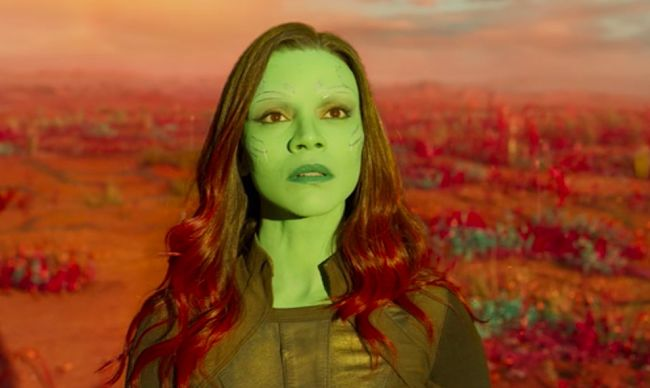
\includegraphics[width=0.49\textwidth]{figures/classifier-hierarchy.jpg}
    \caption{An overview of the proposed ensemble classifier.}
    \label{fig:classifier-hierarchy}
\end{figure}

Most classification tasks are what are called \textbf{flat classification}
meaning there is no hierarchy between the categories or if there is, it is
ignored. Our classification model instead uses the above taxonomy as a guide for \textbf{hierarchical classification} with a top-down approach. In a hierarchical model, multiple classifiers are trained on the same data. Unlike other ensemble methods though, this model trains each classifier with different goals \cite{chou-hierarchical-2003}. Here, we train a classifier per level of the tree. In evaluation, the algorithm follows a classification path, choosing a direction as each level is evaluated. This approach increases overall performance by breaking the classification task into smaller and less complex problems. Additionally, this approach allows us to throw out clearly irrelevant documents early, improving query runtime.

\subsubsection{Risks}
Error propagation is a major issue in this approach and if not managed can ruin the approach outright. Each classifier has some classification error inherent to it and as such a high error on higher level classifiers can seriously impede the efficacy of the system as a whole. We address this through use of probabilistic classifiers, enabling a measure of certainty, and how retrieval of documents is carried out.

Another consideration when working with a hierarchical classifier is whether the lowest level classes have enough examples to train a general model. If too few examples of a low-level class are in the database, the classifiers will begin to overfit. To mitigate this issue, another threshold policy is introduced. This time, the threshold is the minimum number of examples required to allow a classifier to be trained on a certain class. This results in instances of the model trained on a smaller database being less precise in their retrieval.

\subsection{Classification Methods}

\begin{table}[t]
    \centering
    \begin{tabular}{ccc}
         & 250   & 2000  \\ \hline
    DNN  & 0.174 & 0.191 \\
    HDNN & 0.246 & 0.130
    \end{tabular}
    \caption{Classification results of a hierarchical DNN and a standard DNN trained on all 50 classes.}
    \label{tab:classifier}
\end{table}

\begin{itemize}
    % \item Argue non-uniform classifier use
    % \item Argue Probabilistic classifier use
    \item Filtering Classifier
    \item Classifier for Animal Sounds
    \item Classifier for Speech
    \item Classifier for Music
    \item Classifier for Interacting Elements
    \item Teaser of results from experiments
\end{itemize}
Much work has been done in determining what features and classifiers perform the best on audio sub-domains. It is unlikely that in human perception that all different listening tasks are decoded by the same system. Instead there are likely specialized systems that have evolved to best handle specific classification tasks. Thus, the hierarchy has a variety of classifiers specially chosen for their usefulness in each domain.

Probabilistic classifiers are key to mitigating the issue of error propagation in the hierarchical model. While standard classifiers emulate a function of the form y=f(x) with a single result (y) for each input (x), a probabilistic classifier instead emulates conditional distributions of the form P(y|x). We are able to use the resulting probabilities given by a classifier to determine its confidence in the prediction made. We use the confidence to allow normally misclassified results to still be considered. This is done by introducing a threshold (gamma) that must be reached to proceed. Of course, if the threshold is too low then we lose the efficacy of the hierarchical structure in terms of complexity and performance. On the other hand, if the threshold is too high then false negatives will ensure some documents with harder to classify instances of a class will never be retrieved.

% \subsubsection{Annotation Normalization} Annotation normalization is carried
% out on subsets of both the ESC-50 and AudioSet database. Performance is
% measured in terms of execution time, efficiency, and overall annotation
% reduction. The normalization performance is measured against human performance
% and Hsu's normalization results \cite{Hsu2008}. As ESC-50 already has its
% annotations manually normalized, the normalization experiments demonstrate if
% the techniques go too far and overgeneralize. Additionally, it provides a
% clean test-bed for hypernyms to be evaluated. For hypernym sets, we hope to
% have sets that as much as possible attempt to distribute the database across
% them. AudioSet presents a much greater challenge for the low level
% normalization task. These experiments give insight into how the technique
% works at scale and what bottlenecks exist.

/subsection{Filtering Classifier}
The filtering classifier is the root of the classification hierarchy. It is the
first determinant for whether a document should be further considered or discarded when querying. As such, evaluation speed is more important here than on lower levels. The approximate distribution of the classes is summarized in Figure \ref{fig:top-dist} showing that this task proves to be highly computationally intensive with the classes not naturally forming clusters when feature reduced. For the filtering classifier, we use an ensemble of decision tree classifiers referred to as a Random Forest Classifier (RFC).

\textbf{Decision Tree: } A decision tree classifier, as the name implies, is structured as a tree with each node making a decision as to which direction to proceed based on an internal metric, usually either a gini measurement or entropy. This classifier is particularly useful because although the classifier trains more slowly than others, prediction is much faster.

\begin{figure}
    \centering
    \includegraphics[width=0.45\textwidth]{example-image-a}
    \caption{Plot of feature reduced samples from music, animal, speech, and environmental sounds}
    \label{fig:top-dist}
\end{figure}

\subsubsection{General Classifier}
This task is more complex, especially for \textit{Interacting Materials} as it
has a majority of the classes in the database. To evaluate performance with this
classifier we only use the RFC as it is hypothesized that an SVM model would not
be performant.

\subsubsection{Specific Classifier}
As the most complex task in the classification hierarchy, we use two ensemble
classifiers to compare with the DNN implementation. The first has been used in
the other evaluations, RFC, but the second is an AdaBoost classifier. This
classifier uses a collection of weak learners to, as a whole, form a powerful
classification agent.
